\documentclass[border=5pt]{standalone}
\usepackage{tikz}
\usepackage{xcolor}
\usepackage{booktabs}
\usepackage{array}

\definecolor{Garnet}{HTML}{73000A}
\definecolor{NinetyBlack}{HTML}{363636}
\definecolor{SeventyBlack}{HTML}{5C5C5C}
\definecolor{FiftyBlack}{HTML}{A2A2A2}
\definecolor{ThirtyBlack}{HTML}{C7C7C7}
\definecolor{TenBlack}{HTML}{ECECEC}
\definecolor{Atlantic}{HTML}{466A9F}
\definecolor{Sandstorm}{HTML}{FFF2E3}
\definecolor{Congaree}{HTML}{1F414D}

\tikzset{every node/.append style={rounded corners=0pt}}

\begin{document}
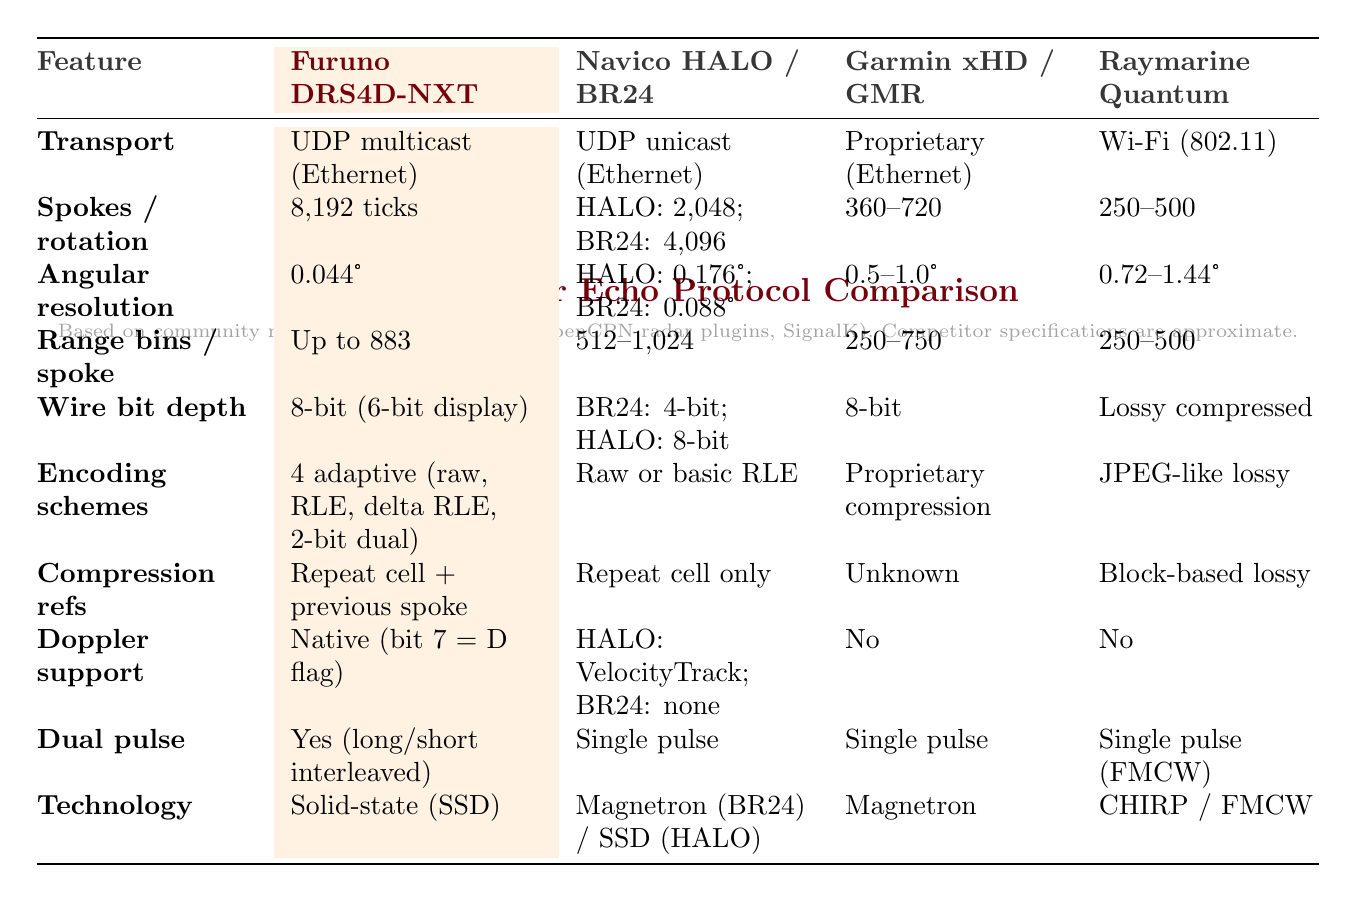
\begin{tikzpicture}
\node[font=\bfseries\large, color=Garnet] at (0, 2.0) {Marine Radar Echo Protocol Comparison};
\node[font=\scriptsize, color=FiftyBlack] at (0, 1.5) {Based on community reverse-engineering efforts (OpenCPN radar plugins, SignalK). Competitor specifications are approximate.};

\node at (0, 0) {
\begin{tabular}{@{} >{\raggedright\arraybackslash}p{2.8cm} >{\columncolor{Sandstorm}\raggedright\arraybackslash}p{3.2cm} >{\raggedright\arraybackslash}p{3.0cm} >{\raggedright\arraybackslash}p{2.8cm} >{\raggedright\arraybackslash}p{2.8cm} @{}}
\toprule
\textbf{\color{NinetyBlack}Feature} &
\textbf{\color{Garnet}Furuno DRS4D-NXT} &
\textbf{\color{NinetyBlack}Navico HALO / BR24} &
\textbf{\color{NinetyBlack}Garmin xHD / GMR} &
\textbf{\color{NinetyBlack}Raymarine Quantum} \\
\midrule
\textbf{Transport} &
UDP multicast (Ethernet) &
UDP unicast (Ethernet) &
Proprietary (Ethernet) &
Wi-Fi (802.11) \\[4pt]
\textbf{Spokes / rotation} &
8{,}192 ticks &
HALO: 2{,}048; BR24: 4{,}096 &
360--720 &
250--500 \\[4pt]
\textbf{Angular resolution} &
0.044\textdegree{} &
HALO: 0.176\textdegree{}; BR24: 0.088\textdegree{} &
0.5--1.0\textdegree{} &
0.72--1.44\textdegree{} \\[4pt]
\textbf{Range bins / spoke} &
Up to 883 &
512--1{,}024 &
250--750 &
250--500 \\[4pt]
\textbf{Wire bit depth} &
8-bit (6-bit display) &
BR24: 4-bit; HALO: 8-bit &
8-bit &
Lossy compressed \\[4pt]
\textbf{Encoding schemes} &
4 adaptive (raw, RLE, delta RLE, 2-bit dual) &
Raw or basic RLE &
Proprietary compression &
JPEG-like lossy \\[4pt]
\textbf{Compression refs} &
Repeat cell + previous spoke &
Repeat cell only &
Unknown &
Block-based lossy \\[4pt]
\textbf{Doppler support} &
Native (bit 7 = D flag) &
HALO: VelocityTrack; BR24: none &
No &
No \\[4pt]
\textbf{Dual pulse} &
Yes (long/short interleaved) &
Single pulse &
Single pulse &
Single pulse (FMCW) \\[4pt]
\textbf{Technology} &
Solid-state (SSD) &
Magnetron (BR24) / SSD (HALO) &
Magnetron &
CHIRP / FMCW \\
\bottomrule
\end{tabular}
};

\end{tikzpicture}
\end{document}
